\documentclass[aspectratio=169,10pt]{beamer}

% Shared Beamer setup for Fall 2026 course slides.
% Clean Cal Poly-inspired theme: no custom class files or uncommon packages.
\mode<presentation>{
  \usetheme{default}
  \usefonttheme{professionalfonts}
}

\definecolor{CalPolyGreen}{HTML}{154734}
\definecolor{CalPolyGold}{HTML}{BD8B13}
\definecolor{CalPolySage}{HTML}{7FA28F}
\definecolor{CalPolyMint}{HTML}{DDF1E7}
\definecolor{CalPolySand}{HTML}{A29F86}
\definecolor{CalPolyBeige}{HTML}{EFEEDE}
\definecolor{DeckInk}{HTML}{1F2933}
\definecolor{DeckMuted}{HTML}{5F6B7A}
\definecolor{DeckSoft}{HTML}{F7F7F5}

\setbeamersize{text margin left=0.55in,text margin right=0.55in}
\setbeamercolor{normal text}{fg=DeckInk,bg=white}
\setbeamercolor{structure}{fg=CalPolyGreen}
\setbeamercolor{title}{fg=white}
\setbeamercolor{frametitle}{fg=CalPolyGreen,bg=white}
\setbeamercolor{block title}{bg=CalPolySage,fg=white}
\setbeamercolor{block body}{bg=CalPolyMint,fg=black}
\setbeamercolor{alerted text}{fg=CalPolyGold}

\setbeamerfont{title}{size=\Huge,series=\bfseries}
\setbeamerfont{frametitle}{size=\Large,series=\bfseries}
\setbeamerfont{block title}{size=\normalsize,series=\bfseries}

\setbeamertemplate{navigation symbols}{}
\setbeamertemplate{itemize item}{\color{CalPolyGold}$\blacktriangleright$}
\setbeamertemplate{itemize subitem}{\color{CalPolyGreen}$\bullet$}
\setbeamertemplate{footline}{
  \hfill{\color{DeckMuted}\scriptsize\insertframenumber/\inserttotalframenumber}
  \hspace{0.18in}\vspace{0.12in}
}
\setbeamertemplate{frametitle}{
  \vspace{0.18in}
  \hspace{0.02in}\insertframetitle\par
  \vspace{0.08in}
  \noindent\makebox[\linewidth][l]{%
    {\color{CalPolyGold}\rule{0.55in}{2pt}}%
    {\color{CalPolyGreen}\rule{\dimexpr\linewidth-0.55in\relax}{2pt}}%
  }
}

\newcommand{\CourseNumber}{Course}
\newcommand{\CourseTitle}{Course Title}
\newcommand{\LectureNumber}{0}
\newcommand{\LectureTitle}{Lecture Title}
\newcommand{\LectureDate}{Date}
\newcommand{\CourseUnit}{Unit}

\newcommand{\coursenumber}[1]{\renewcommand{\CourseNumber}{#1}}
\newcommand{\coursetitle}[1]{\renewcommand{\CourseTitle}{#1}}
\newcommand{\lecturenumber}[1]{\renewcommand{\LectureNumber}{#1}}
\newcommand{\lecturetitle}[1]{\renewcommand{\LectureTitle}{#1}}
\newcommand{\lecturedate}[1]{\renewcommand{\LectureDate}{#1}}
\newcommand{\courseunit}[1]{\renewcommand{\CourseUnit}{#1}}

\author{Kirk Duran}
\institute{California Polytechnic State University, San Luis Obispo}
\date{\LectureDate}

\newcommand{\makedecktitle}{
  \begingroup
  \setbeamercolor{background canvas}{bg=CalPolyGreen}
  \begin{frame}[plain]
    \vfill
    \begin{center}
      {\usebeamerfont{title}\color{white}\LectureTitle\par}
      \vspace{0.18in}
      {\Large\color{white}Lecture \LectureNumber\par}
    \end{center}
    \vfill
    \noindent{\color{white}\rule{\linewidth}{1.2pt}}\par
    \vspace{0.08in}
    \noindent\colorbox{CalPolyGold}{\makebox[0.24\linewidth][c]{\color{white}\Large\CourseNumber}}
    \hspace{0.12in}{\color{white}\Large Kirk Duran}
  \end{frame}
  \endgroup
}

\newenvironment{keyidea}{\begin{block}{Key idea}}{\end{block}}
\newenvironment{activity}{\begin{block}{In class}}{\end{block}}
\newenvironment{cpdefinition}{\begin{block}{Definition}}{\end{block}}
\newenvironment{exampleblockcp}{
  \begingroup
  \setbeamercolor{block title}{bg=CalPolySand,fg=white}
  \setbeamercolor{block body}{bg=CalPolyBeige,fg=black}
  \begin{block}{Example}
}{
  \end{block}
  \endgroup
}

\newcommand{\imageplaceholder}[2][0.3in]{%
  \noindent\makebox[\linewidth][c]{%
    \fcolorbox{CalPolySage}{CalPolyBeige}{%
      \parbox[c][#1][c]{0.86\linewidth}{%
        \centering
        {\color{DeckMuted}\scriptsize Image placeholder: }%
        {\color{DeckInk}\scriptsize\ttfamily\detokenize{#2}}%
      }%
    }%
  }%
}

\newcommand{\sectionframe}[1]{
  \begingroup
  \setbeamercolor{background canvas}{bg=CalPolyGreen}
  \begin{frame}[plain]
    \vfill
    {\color{white}\LARGE\bfseries #1\par}
    \vspace{0.18in}
    {\color{CalPolyGold}\rule{0.22\paperwidth}{3pt}}
    {\color{white}\rule{0.62\paperwidth}{3pt}}
    \vfill
  \end{frame}
  \endgroup
}

\newcommand{\placeholdernote}{
  \begin{block}{Placeholder}
    Replace these bullets with the final lecture material, examples, and in-class activities.
  \end{block}
}


\usepackage{tikz}
\usetikzlibrary{arrows.meta,positioning,shapes.geometric,calc}

\graphicspath{{../assets/lecture-22/}}

\newcommand{\lectureimage}[2][1.75in]{%
  \IfFileExists{../assets/lecture-22/#2}{%
    \includegraphics[width=\linewidth,height=#1,keepaspectratio]{#2}%
  }{}%
}

\newcommand{\lectureplaceholder}[2][2.35in]{%
  \begin{center}
    \fbox{%
      \begin{minipage}[c][#1][c]{0.90\linewidth}
        \centering
        \small\textit{#2}
      \end{minipage}%
    }
  \end{center}%
}

\setbeamersize{text margin left=0.42in,text margin right=0.42in}

\coursenumber{CS 4880}
\coursetitle{Artificial Intelligence}
\lecturenumber{22}
\lecturetitle{Utility Theory and Decision Networks}
\lecturedate{October 16, 2026}
\courseunit{Temporal and Decision Reasoning}

\begin{document}

% Estimated pacing: 50--55 minutes
% From belief to action: 8 min
% Utility and expected utility: 15 min
% Multiattribute utility + design tradeoffs: 8 min
% Decision networks: 8 min
% Value of information: 8 min
% Repeated myopic decisions + MDP bridge: 8 min

% -----------------------------------------------------------------------------
% Slide 1
% -----------------------------------------------------------------------------
\makedecktitle

\section{From Knowing to Choosing}

% -----------------------------------------------------------------------------
% Slide 2
% -----------------------------------------------------------------------------
\begin{frame}[shrink=10]{Last Time: The Robot Estimated Its State}
  Dynamic Bayesian networks and filters gave the robot a belief about the current world:
  \[
    bel_t(x)=P(X_t=x\mid z_{1:t}).
  \]

  \begin{itemize}
    \item HMMs represented compact discrete hidden state.
    \item Kalman filters represented linear-Gaussian continuous state.
    \item Particle filters represented flexible beliefs using weighted samples.
  \end{itemize}

  \begin{block}{Lecture 21 question}
    ``Where am I, and what is happening around me?''
  \end{block}

  \begin{keyidea}
    State estimation gives the agent beliefs about the world; decision theory uses those beliefs to choose actions.
  \end{keyidea}
\end{frame}

% -----------------------------------------------------------------------------
% Slide 3
% -----------------------------------------------------------------------------
\begin{frame}[shrink=10]{The Robot Is No Longer Following a Fixed Route}
  The delivery robot no longer receives a precomputed sequence of moves.

  At every control cycle it must choose what to do next based on:
  \begin{itemize}
    \item its current position belief;
    \item uncertain obstacles and pedestrian traffic;
    \item remaining delivery time;
    \item battery state;
    \item current task priority.
  \end{itemize}

  \lectureimage[2.0in]{slide3.png}

  \begin{keyidea}
    The planning problem has moved inside the loop: estimate the current situation, choose the next action, observe the result, repeat.
  \end{keyidea}
\end{frame}

% -----------------------------------------------------------------------------
% Slide 4
% -----------------------------------------------------------------------------
\begin{frame}[shrink=10]{A Good State Estimate Still Does Not Tell Us What to Do}
  Suppose the robot believes
  \[
    P(Blocked)=0.35,
    \qquad
    P(Clear)=0.65.
  \]

  That belief does not answer:
  \begin{itemize}
    \item Is the shortcut worth attempting?
    \item Should the robot take a longer but safer detour?
    \item Is it worth waiting for congestion to clear?
    \item Is another sensor scan worth the time and energy?
  \end{itemize}

  \begin{keyidea}
    Probability ranks how plausible outcomes are. Decision making also requires preferences over those outcomes.
  \end{keyidea}
\end{frame}

% -----------------------------------------------------------------------------
% Slide 5
% -----------------------------------------------------------------------------
\begin{frame}[shrink=10]{The New Control Loop}
  \begin{center}
    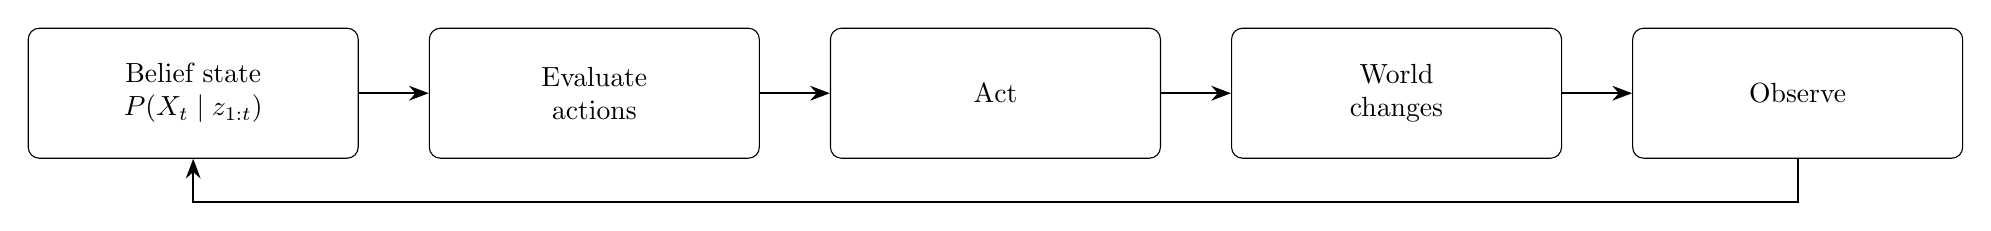
\begin{tikzpicture}[node distance=0.35in,every node/.style={draw,rounded corners,align=center,minimum height=0.65in,minimum width=1.65in}]
      \node (b) {Belief state\\$P(X_t\mid z_{1:t})$};
      \node[right=of b] (e) {Evaluate\\actions};
      \node[right=of e] (a) {Act};
      \node[right=of a] (w) {World\\changes};
      \node[right=of w] (o) {Observe};
      \draw[-{Stealth[length=2.5mm]},thick] (b)--(e);
      \draw[-{Stealth[length=2.5mm]},thick] (e)--(a);
      \draw[-{Stealth[length=2.5mm]},thick] (a)--(w);
      \draw[-{Stealth[length=2.5mm]},thick] (w)--(o);
      \draw[-{Stealth[length=2.5mm]},thick] (o.south) |- ++(0,-0.55) -| (b.south);
    \end{tikzpicture}
  \end{center}

  The robot repeatedly converts a current belief into a next action.

  \begin{keyidea}
    Decision theory turns the robot from a passive estimator into an agent that continually converts beliefs into actions.
  \end{keyidea}
\end{frame}

% -----------------------------------------------------------------------------
% Slide 6
% -----------------------------------------------------------------------------
\begin{frame}[shrink=10]{At One Campus Intersection, the Robot Has Several Actions}
  \begin{columns}[T,onlytextwidth]
    \begin{column}{0.23\textwidth}
      \begin{block}{Shortcut}
        Fastest route. May be blocked by a crowd or maintenance cart.
      \end{block}
    \end{column}
    \begin{column}{0.23\textwidth}
      \begin{block}{Detour}
        Longer route around the building. Usually clear and predictable.
      \end{block}
    \end{column}
    \begin{column}{0.23\textwidth}
      \begin{block}{Wait}
        Spend time while congestion may clear.
      \end{block}
    \end{column}
    \begin{column}{0.23\textwidth}
      \begin{block}{Scan}
        Pause for a better sensor reading before committing.
      \end{block}
    \end{column}
  \end{columns}

  \begin{keyidea}
    An action is valuable because of the distribution of outcomes it creates---not because its name sounds desirable.
  \end{keyidea}
\end{frame}

% -----------------------------------------------------------------------------
% Slide 7
% -----------------------------------------------------------------------------
\begin{frame}[shrink=10]{Probability Alone Cannot Choose Between Actions}
  The current belief is
  \[
    P(Clear)=0.65,
    \qquad
    P(Blocked)=0.35.
  \]

  But should the robot take the shortcut?

  We still need to know:
  \begin{itemize}
    \item how valuable a fast successful shortcut is;
    \item how costly a blocked attempt is;
    \item how much delay the detour causes;
    \item how strongly the system prefers safety, time, and energy conservation.
  \end{itemize}

  \begin{keyidea}
    Choosing an action requires both a probabilistic model of consequences and a preference model over those consequences.
  \end{keyidea}
\end{frame}

\section{Utility Theory}

% -----------------------------------------------------------------------------
% Slide 8
% -----------------------------------------------------------------------------
\begin{frame}[shrink=10]{Utility Turns Preferences into a Numerical Model}
  A \textbf{utility function} assigns a numerical value to an outcome:
  \[
    U(o): outcome \rightarrow \mathbb{R}.
  \]

  Example preference ordering:
  \[
    U(\text{fast safe delivery})
    > U(\text{safe detour})
    > U(\text{blocked attempt}).
  \]

  \begin{keyidea}
    Utility is a compact numerical representation of the agent's preferences over outcomes.
  \end{keyidea}
\end{frame}

% -----------------------------------------------------------------------------
% Slide 9
% -----------------------------------------------------------------------------
\begin{frame}[shrink=10]{Only Relative Utility Matters}
  Utility is not a physical measurement like meters or joules.

  If a positive affine transformation is applied,
  \[
    U'(o)=aU(o)+b,
    \qquad a>0,
  \]
  the same preference ordering is preserved.

  Example:
  \[
    U(\text{fast safe})=80,
    \quad U(\text{detour})=45,
    \quad U(\text{blocked})=-60.
  \]

  \begin{keyidea}
    Utility values are meaningful through preference comparisons and tradeoffs, not as standalone units.
  \end{keyidea}
\end{frame}

% -----------------------------------------------------------------------------
% Slide 10
% -----------------------------------------------------------------------------
\begin{frame}[shrink=10]{Under Uncertainty, Use Expected Utility}
  For an action $a$ with possible outcomes $o$,
  \[
    EU(a)=\sum_o P(o\mid a)U(o).
  \]

  A rational expected-utility decision rule chooses
  \[
    a^*=\arg\max_a EU(a).
  \]

  \begin{columns}[T,onlytextwidth]
    \begin{column}{0.31\textwidth}
      \begin{block}{Probability}
        How likely is each outcome if I choose this action?
      \end{block}
    \end{column}
    \begin{column}{0.31\textwidth}
      \begin{block}{Utility}
        How desirable is each outcome?
      \end{block}
    \end{column}
    \begin{column}{0.31\textwidth}
      \begin{block}{Decision}
        Choose the action with greatest expected utility.
      \end{block}
    \end{column}
  \end{columns}

  \begin{keyidea}
    Expected utility weights each possible consequence by both its probability and its desirability.
  \end{keyidea}
\end{frame}

% -----------------------------------------------------------------------------
% Slide 11
% -----------------------------------------------------------------------------
\begin{frame}[shrink=10]{Worked Decision: Shortcut or Detour?}
  Current belief:
  \[
    P(Clear)=0.65,
    \qquad
    P(Blocked)=0.35.
  \]

  Utility model:
  \[
    U(Shortcut,Clear)=80,
  \]
  \[
    U(Shortcut,Blocked)=-60,
  \]
  \[
    U(Detour)=45.
  \]

  \begin{keyidea}
    The action with the most likely good outcome is not necessarily the action with the highest expected utility.
  \end{keyidea}
\end{frame}

% -----------------------------------------------------------------------------
% Slide 12
% -----------------------------------------------------------------------------
\begin{frame}[shrink=10]{Expected Utility of the Shortcut}
  \[
    EU(Shortcut)
      =0.65(80)+0.35(-60)
  \]
  \[
      =52-21
      =31.
  \]

  The shortcut is more likely to be clear than blocked, but the blocked outcome is costly enough to reduce its expected utility substantially.

  \begin{keyidea}
    Expected utility combines the upside and downside of an action in one probability-weighted quantity.
  \end{keyidea}
\end{frame}

% -----------------------------------------------------------------------------
% Slide 13
% -----------------------------------------------------------------------------
\begin{frame}[shrink=10]{Expected Utility of the Detour}
  For the simplified example, the detour is predictable:
  \[
    EU(Detour)=45.
  \]

  Therefore
  \[
    45>31.
  \]

  The rational one-step choice is the detour.

  \begin{keyidea}
    Rational choice is about expected preference, not simply choosing the most probable outcome.
  \end{keyidea}
\end{frame}

% -----------------------------------------------------------------------------
% Slide 14
% -----------------------------------------------------------------------------
\begin{frame}[shrink=10]{Most Likely Outcome $\neq$ Best Action}
  \begin{columns}[T,onlytextwidth]
    \begin{column}{0.47\textwidth}
      \begin{block}{Maximum-probability thinking}
        ``The shortcut is 65\% likely to be clear, so take the shortcut.''

        This ignores how bad the 35\% failure case is.
      \end{block}
    \end{column}
    \begin{column}{0.47\textwidth}
      \begin{block}{Expected-utility thinking}
        ``The shortcut is often faster, but failure is costly enough that the detour has higher expected utility.''
      \end{block}
    \end{column}
  \end{columns}

  \begin{keyidea}
    Decision theory separates probability from preference so rare but severe outcomes can matter appropriately.
  \end{keyidea}
\end{frame}

% -----------------------------------------------------------------------------
% Slide 15
% -----------------------------------------------------------------------------
\begin{frame}[shrink=10]{A Robot Usually Has More Than One Objective}
  The robot may simultaneously care about:
  \begin{itemize}
    \item travel time;
    \item energy consumption;
    \item collision and pedestrian risk;
    \item progress toward completing the delivery;
    \item reliability and schedule slack.
  \end{itemize}

  These objectives can conflict.

  \begin{keyidea}
    Real decision systems often optimize several competing attributes, so the utility model must make those tradeoffs explicit.
  \end{keyidea}
\end{frame}

% -----------------------------------------------------------------------------
% Slide 16
% -----------------------------------------------------------------------------
\begin{frame}[shrink=10]{One Engineering Approximation: Multiattribute Utility}
  A simple model is a weighted sum:
  \[
    U(o)=w_tu_t(o)+w_eu_e(o)+w_su_s(o)+w_pu_p(o).
  \]

  The weights encode the relative importance of time, energy, safety, and task progress.

  \begin{block}{Important modeling assumption}
    A weighted sum is convenient, but it assumes the attributes can be combined in this way. Real preference interactions may require a richer utility model.
  \end{block}

  \begin{keyidea}
    Utility design is a modeling choice: convenient mathematical structure buys simplicity but may hide real preference interactions.
  \end{keyidea}
\end{frame}

% -----------------------------------------------------------------------------
% Slide 17
% -----------------------------------------------------------------------------
\begin{frame}[shrink=10]{Changing the Weights Can Change the Robot's Behavior}
  \begin{columns}[T,onlytextwidth]
    \begin{column}{0.31\textwidth}
      \begin{block}{Time-heavy}
        Large penalty for delay. The robot accepts more uncertainty to preserve deadline slack.
      \end{block}
    \end{column}
    \begin{column}{0.31\textwidth}
      \begin{block}{Energy-heavy}
        Battery is scarce. The robot avoids steep ramps, long scans, and unnecessary detours.
      \end{block}
    \end{column}
    \begin{column}{0.31\textwidth}
      \begin{block}{Safety-heavy}
        The robot prefers conservative routes through uncertain pedestrian traffic.
      \end{block}
    \end{column}
  \end{columns}

  \begin{keyidea}
    The same probability model can produce very different behavior under different utility functions.
  \end{keyidea}
\end{frame}

% -----------------------------------------------------------------------------
% Slide 18
% -----------------------------------------------------------------------------
\begin{frame}[shrink=10]{Not Every Requirement Should Be ``Just Another Weight''}
  Weighted utilities make tradeoffs possible by design.

  But some requirements may instead be treated as \textbf{hard constraints}:
  \begin{itemize}
    \item exclude actions that violate safety envelopes;
    \item enforce legal or operational limits;
    \item optimize utility only among feasible actions.
  \end{itemize}

  This matters when a tiny probability of a catastrophic outcome should not be casually exchanged for a small improvement in speed.

  \begin{keyidea}
    Utility maximization is only as sensible as the objectives, constraints, and action set supplied to it.
  \end{keyidea}
\end{frame}

\section{Decision Networks}

% -----------------------------------------------------------------------------
% Slide 19
% -----------------------------------------------------------------------------
\begin{frame}[shrink=10]{Decision Networks Add Actions and Preferences to Bayes Nets}
  A \textbf{decision network} or \textbf{influence diagram} contains three node types:

  \begin{columns}[T,onlytextwidth]
    \begin{column}{0.31\textwidth}
      \begin{block}{Chance node}
        Uncertain random variable.

        Example: shortcut blocked?
      \end{block}
    \end{column}
    \begin{column}{0.31\textwidth}
      \begin{block}{Decision node}
        Choice controlled by the agent.

        Example: shortcut, detour, scan, wait.
      \end{block}
    \end{column}
    \begin{column}{0.31\textwidth}
      \begin{block}{Utility node}
        Preference over resulting outcomes.

        Example: time + energy + safety + progress.
      \end{block}
    \end{column}
  \end{columns}

  \begin{keyidea}
    A decision network combines uncertainty, controllable choices, and utility in one graphical model.
  \end{keyidea}
\end{frame}

% -----------------------------------------------------------------------------
% Slide 20
% -----------------------------------------------------------------------------
\begin{frame}[shrink=10]{Robot Decision Network: One Next-Move Choice}
  \begin{center}
    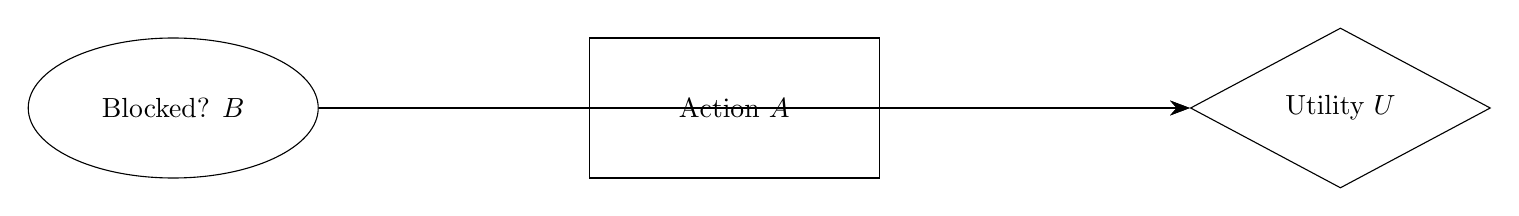
\begin{tikzpicture}[node distance=1.35in]
      \node[draw,ellipse,minimum width=1.45in,minimum height=0.70in] (b) {Blocked? $B$};
      \node[draw,rectangle,right=of b,minimum width=1.45in,minimum height=0.70in] (a) {Action $A$};
      \node[draw,diamond,right=1.55in of a,aspect=2.2,minimum width=1.5in,minimum height=0.8in] (u) {Utility $U$};
      \draw[-{Stealth[length=2.5mm]},thick] (b)--(u);
      \draw[-{Stealth[length=2.5mm]},thick] (a)--(u);
    \end{tikzpicture}
  \end{center}

  The world state affects the outcome. The chosen action also affects the outcome. Utility evaluates the combination.

  \begin{keyidea}
    Decision networks make the separation between ``what the world may do'' and ``what the agent may choose'' explicit.
  \end{keyidea}
\end{frame}

% -----------------------------------------------------------------------------
% Slide 21
% -----------------------------------------------------------------------------
\begin{frame}[shrink=10]{Information Arcs Mean ``Known Before the Decision''}
  Suppose a sensor reading $Z$ is available before the action is chosen.

  \begin{center}
    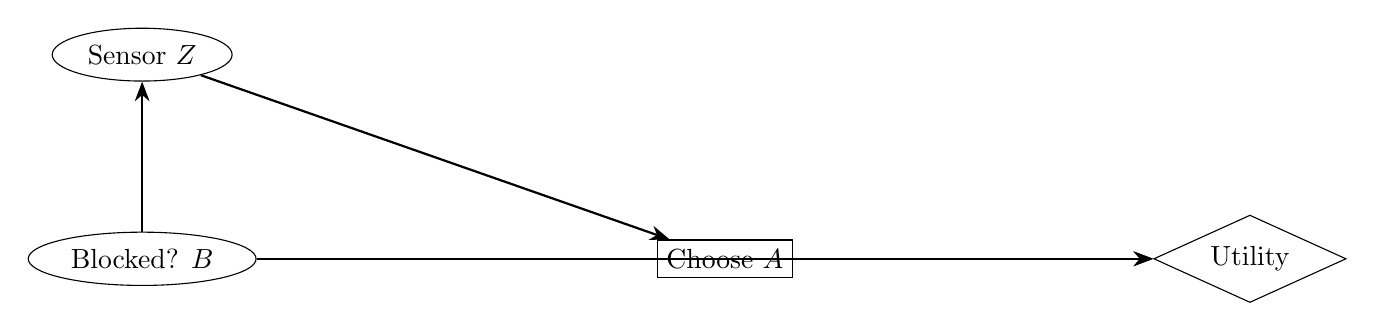
\begin{tikzpicture}[node distance=1.25in]
      \node[draw,ellipse] (b) {Blocked? $B$};
      \node[draw,ellipse,above=0.75in of b] (z) {Sensor $Z$};
      \node[draw,rectangle,right=2.0in of b] (a) {Choose $A$};
      \node[draw,diamond,right=1.8in of a,aspect=2.2] (u) {Utility};
      \draw[-{Stealth[length=2.5mm]},thick] (b)--(z);
      \draw[-{Stealth[length=2.5mm]},thick] (z)--(a);
      \draw[-{Stealth[length=2.5mm]},thick] (b)--(u);
      \draw[-{Stealth[length=2.5mm]},thick] (a)--(u);
    \end{tikzpicture}
  \end{center}

  An arrow into a decision node indicates information available at decision time; it is not a CPT for the decision itself.

  \begin{keyidea}
    The decision can condition on observations the agent has already seen.
  \end{keyidea}
\end{frame}

% -----------------------------------------------------------------------------
% Slide 22
% -----------------------------------------------------------------------------
\begin{frame}[shrink=10]{Evaluating a Decision Network: Sum at Chance, Max at Decision}
  At a chance variable, average over possible outcomes:
  \[
    EU(a)=\sum_o P(o\mid a)U(o).
  \]

  At the decision variable, choose the maximizing action:
  \[
    a^*=\arg\max_a EU(a).
  \]

  The result is a decision rule or policy for the current decision context.

  \begin{keyidea}
    Probabilistic inference supplies the distribution; decision optimization selects the maximizing action.
  \end{keyidea}
\end{frame}

% -----------------------------------------------------------------------------
% Slide 23
% -----------------------------------------------------------------------------
\begin{frame}[shrink=10]{The Belief State from Lecture 21 Plugs Directly Into the Decision}
  \begin{center}
    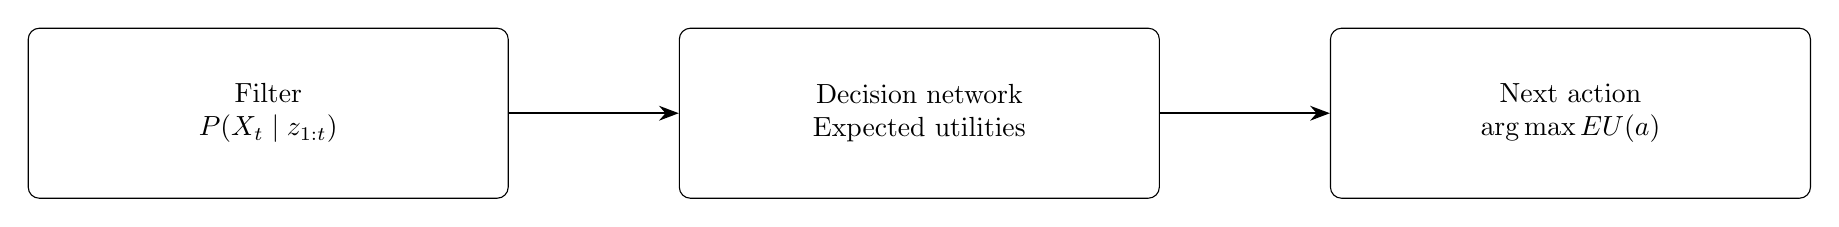
\begin{tikzpicture}[node distance=0.85in,every node/.style={draw,rounded corners,align=center,minimum width=2.4in,minimum height=0.85in}]
      \node (f) {Filter\\$P(X_t\mid z_{1:t})$};
      \node[right=of f] (d) {Decision network\\Expected utilities};
      \node[right=of d] (a) {Next action\\$\arg\max EU(a)$};
      \draw[-{Stealth[length=2.5mm]},thick] (f)--(d);
      \draw[-{Stealth[length=2.5mm]},thick] (d)--(a);
    \end{tikzpicture}
  \end{center}

  State estimation and decision making are not competing algorithms. The current belief is an input to the decision.

  \begin{keyidea}
    The agent acts on what it currently believes---not on an inaccessible perfect state of the world.
  \end{keyidea}
\end{frame}

% -----------------------------------------------------------------------------
% Slide 24
% -----------------------------------------------------------------------------
\begin{frame}[shrink=10]{One-Step Decision Procedure}
  At each control cycle:
  \begin{enumerate}
    \item update the belief state $b_t$;
    \item generate feasible actions $A(b_t)$;
    \item predict possible outcomes for each action;
    \item compute expected utility for each action;
    \item execute $\arg\max_a EU(a)$.
  \end{enumerate}

  \begin{keyidea}
    This is a rational one-step controller: repeatedly choose the action with the best expected immediate outcome under the current belief.
  \end{keyidea}
\end{frame}

\section{Value of Information}

% -----------------------------------------------------------------------------
% Slide 25
% -----------------------------------------------------------------------------
\begin{frame}[shrink=10]{Sometimes ``Get More Information'' Is Itself an Action}
  \begin{columns}[T,onlytextwidth]
    \begin{column}{0.47\textwidth}
      \begin{block}{Act now}
        Choose shortcut or detour using the current belief.

        No sensing delay, but uncertainty remains high.
      \end{block}
    \end{column}
    \begin{column}{0.47\textwidth}
      \begin{block}{Scan first}
        Pause for a better sensor reading, update the belief, then choose.

        Costs time and energy, but may improve the eventual action.
      \end{block}
    \end{column}
  \end{columns}

  \begin{keyidea}
    Information has instrumental value when it can improve the action the robot chooses afterward.
  \end{keyidea}
\end{frame}

% -----------------------------------------------------------------------------
% Slide 26
% -----------------------------------------------------------------------------
\begin{frame}[shrink=10]{Value of Information: Will a Better Measurement Change the Decision?}
  Current belief:
  \[
    P(Blocked)=0.35.
  \]

  Without another measurement, the robot chooses the detour with utility $45$.

  A short active scan costs $5$ utility units and has sensor model
  \[
    P(+\mid Blocked)=0.90,
    \qquad
    P(+\mid Clear)=0.10.
  \]

  Is the scan worth its cost?

  \begin{keyidea}
    The value of information depends on how the observation changes downstream decisions, not only on sensor accuracy.
  \end{keyidea}
\end{frame}

% -----------------------------------------------------------------------------
% Slide 27
% -----------------------------------------------------------------------------
\begin{frame}[shrink=10]{The Scan Produces Two Possible Belief Updates}
  First,
  \[
    P(+)=0.90(0.35)+0.10(0.65)=0.38.
  \]

  Then Bayes' rule gives
  \[
    P(Blocked\mid +)
      =\frac{0.90(0.35)}{0.38}
      \approx 0.829,
  \]
  while
  \[
    P(Blocked\mid -)
      =\frac{0.10(0.35)}{0.62}
      \approx 0.056.
  \]

  \begin{keyidea}
    A useful observation partitions the future decision into different belief states that may justify different actions.
  \end{keyidea}
\end{frame}

% -----------------------------------------------------------------------------
% Slide 28
% -----------------------------------------------------------------------------
\begin{frame}[shrink=10]{After the Scan, the Best Action Depends on the Observation}
  If the scan is positive:
  \[
    P(Blocked\mid +)\approx0.829,
  \]
  so the shortcut has expected utility approximately $-36$ and the robot chooses the detour.

  If the scan is negative:
  \[
    P(Blocked\mid -)\approx0.056,
  \]
  so the shortcut has expected utility approximately $72.1$ and the robot chooses the shortcut.

  \begin{keyidea}
    The scan is valuable because different observations lead to different actions.
  \end{keyidea}
\end{frame}

% -----------------------------------------------------------------------------
% Slide 29
% -----------------------------------------------------------------------------
\begin{frame}[shrink=10]{Expected Value of the Scan}
  Before subtracting sensing cost,
  \[
    EV(Scan)
      =0.38(45)+0.62(72.1)
      \approx 61.8.
  \]

  Subtract the cost of scanning:
  \[
    61.8-5=56.8.
  \]

  Without scanning, the best action has value $45$.

  Therefore the net value of scanning is
  \[
    56.8-45=+11.8.
  \]

  \begin{keyidea}
    Information is worth acquiring when its expected improvement in decision quality exceeds its sensing cost.
  \end{keyidea}
\end{frame}

% -----------------------------------------------------------------------------
% Slide 30
% -----------------------------------------------------------------------------
\begin{frame}[shrink=10]{Information Can Be Accurate and Still Have Zero Decision Value}
  \begin{columns}[T,onlytextwidth]
    \begin{column}{0.47\textwidth}
      \begin{block}{Observation changes the action}
        Positive $\rightarrow$ detour

        Negative $\rightarrow$ shortcut

        The information can have positive decision value.
      \end{block}
    \end{column}
    \begin{column}{0.47\textwidth}
      \begin{block}{Same action either way}
        Positive $\rightarrow$ detour

        Negative $\rightarrow$ detour

        Even a very accurate observation may have little decision value.
      \end{block}
    \end{column}
  \end{columns}

  \begin{keyidea}
    Decision-relevant information is valuable because of its effect on action choice, not because reducing uncertainty is automatically useful.
  \end{keyidea}
\end{frame}

\section{Repeating the Decision}

% -----------------------------------------------------------------------------
% Slide 31
% -----------------------------------------------------------------------------
\begin{frame}[shrink=10]{Now Put the Decision Back Inside the Robot Loop}
  \begin{center}
    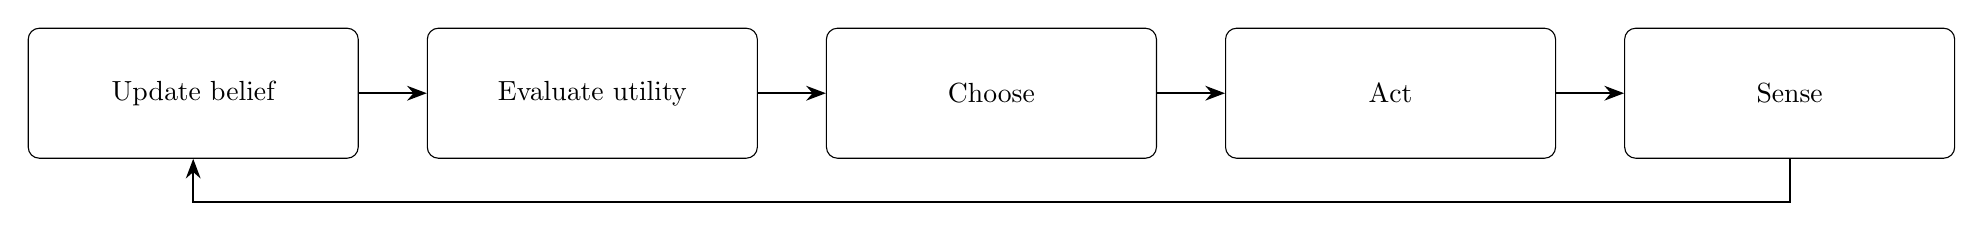
\begin{tikzpicture}[node distance=0.34in,every node/.style={draw,rounded corners,align=center,minimum width=1.65in,minimum height=0.65in}]
      \node (b) {Update belief};
      \node[right=of b] (u) {Evaluate utility};
      \node[right=of u] (c) {Choose};
      \node[right=of c] (a) {Act};
      \node[right=of a] (s) {Sense};
      \draw[-{Stealth[length=2.5mm]},thick] (b)--(u);
      \draw[-{Stealth[length=2.5mm]},thick] (u)--(c);
      \draw[-{Stealth[length=2.5mm]},thick] (c)--(a);
      \draw[-{Stealth[length=2.5mm]},thick] (a)--(s);
      \draw[-{Stealth[length=2.5mm]},thick] (s.south) |- ++(0,-0.55) -| (b.south);
    \end{tikzpicture}
  \end{center}

  This loop may execute dozens or hundreds of times during one delivery.

  \begin{keyidea}
    A decision network can be reevaluated every control cycle using the robot's newest belief state.
  \end{keyidea}
\end{frame}

% -----------------------------------------------------------------------------
% Slide 32
% -----------------------------------------------------------------------------
\begin{frame}[shrink=10]{This Gives Us a Myopic Decision Controller}
  \begin{block}{One-step controller}
    \ttfamily\small
    while delivery not complete:\\
    \quad b\_t = update\_belief(sensor\_data)\\
    \quad actions = feasible\_actions(b\_t)\\
    \quad for a in actions:\\
    \qquad EU[a] = expected\_immediate\_utility(a,b\_t)\\
    \quad execute(argmax\_a EU[a])
  \end{block}

  It is \textbf{myopic} because it optimizes what is best now without yet including the value of future states and future actions.

  \begin{keyidea}
    Repeated one-step optimization is a useful reactive strategy, but repeated local optimality does not guarantee globally good behavior.
  \end{keyidea}
\end{frame}

% -----------------------------------------------------------------------------
% Slide 33
% -----------------------------------------------------------------------------
\begin{frame}[shrink=10]{Failure Mode: Locally Rational Actions Can Oscillate}
  Imagine two similar corridors whose estimated congestion changes slightly with each noisy scan.

  \begin{enumerate}
    \item At time $t$, left has slightly higher immediate expected utility $\rightarrow$ turn left.
    \item At time $t+1$, a new reading makes right slightly better $\rightarrow$ turn right.
    \item At time $t+2$, noise flips the preference again $\rightarrow$ turn left.
  \end{enumerate}

  \[
    Left \leftrightarrow Right \leftrightarrow Left \leftrightarrow \cdots
  \]

  \begin{keyidea}
    A controller that only asks ``what is best this instant?'' can thrash when actions have switching costs or delayed effects.
  \end{keyidea}
\end{frame}

% -----------------------------------------------------------------------------
% Slide 34
% -----------------------------------------------------------------------------
\begin{frame}[shrink=10]{Failure Mode: The Best Immediate Move Can Create a Bad Future}
  \begin{columns}[T,onlytextwidth]
    \begin{column}{0.47\textwidth}
      \begin{block}{Narrow shortcut}
        Immediate utility: $+30$.

        Moves quickly toward the destination, but enters a courtyard with one exit and frequent congestion.
      \end{block}
    \end{column}
    \begin{column}{0.47\textwidth}
      \begin{block}{Wider detour}
        Immediate utility: $+20$.

        Looks worse right now, but preserves several future route choices.
      \end{block}
    \end{column}
  \end{columns}

  \begin{keyidea}
    Actions do not merely produce immediate outcomes---they change which states and choices will be available later.
  \end{keyidea}
\end{frame}

% -----------------------------------------------------------------------------
% Slide 35
% -----------------------------------------------------------------------------
\begin{frame}[shrink=10]{The Question Has Changed Again}
  So far the robot chooses
  \[
    a_t^*=\arg\max_a EU(a\mid b_t).
  \]

  But repeated autonomous control asks something stronger:

  \begin{center}
    \Large\textbf{What action is best when I also care about the future states and future decisions it creates?}
  \end{center}

  \begin{keyidea}
    Once actions influence future opportunities, rational decision making must reason across sequences of states and actions.
  \end{keyidea}
\end{frame}

% -----------------------------------------------------------------------------
% Slide 36
% -----------------------------------------------------------------------------
\begin{frame}[shrink=10]{Next: Markov Decision Processes}
  Lecture 23 will formalize the repeated decision problem with:

  \begin{itemize}
    \item \textbf{states}: what situation is the robot in?
    \item \textbf{actions}: what can the robot do?
    \item \textbf{transitions}: where might each action take it?
    \item \textbf{rewards}: what immediate signal does a transition produce?
    \item \textbf{policy}: what should the robot do in every state?
  \end{itemize}

  \begin{keyidea}
    Decision networks choose under uncertainty; MDPs will formalize repeated decisions whose consequences propagate into the future.
  \end{keyidea}
\end{frame}

% -----------------------------------------------------------------------------
% Slide 37
% -----------------------------------------------------------------------------
\begin{frame}[shrink=10]{The Whole Unit Now Forms One Pipeline}
  \begin{center}
    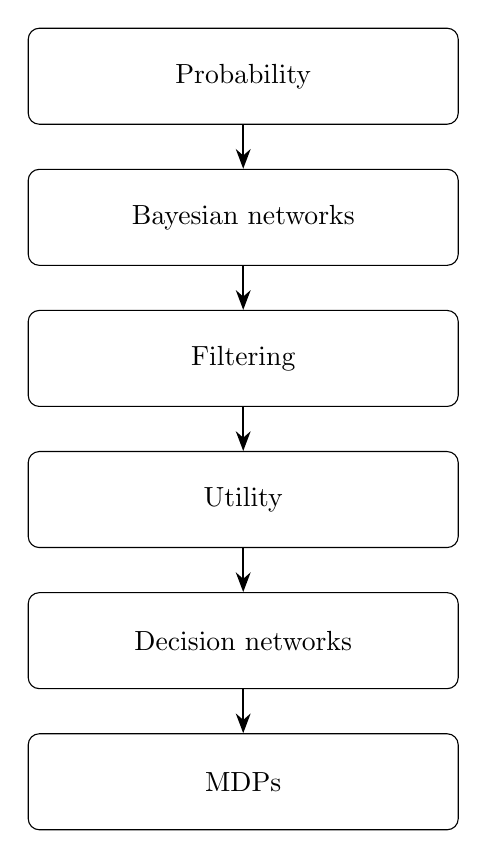
\begin{tikzpicture}[node distance=0.22in,every node/.style={draw,rounded corners,align=center,minimum width=2.15in,minimum height=0.48in}]
      \node (p) {Probability};
      \node[below=of p] (bn) {Bayesian networks};
      \node[below=of bn] (f) {Filtering};
      \node[below=of f] (u) {Utility};
      \node[below=of u] (dn) {Decision networks};
      \node[below=of dn] (m) {MDPs};
      \draw[-{Stealth[length=2.5mm]},thick] (p)--(bn);
      \draw[-{Stealth[length=2.5mm]},thick] (bn)--(f);
      \draw[-{Stealth[length=2.5mm]},thick] (f)--(u);
      \draw[-{Stealth[length=2.5mm]},thick] (u)--(dn);
      \draw[-{Stealth[length=2.5mm]},thick] (dn)--(m);
    \end{tikzpicture}
  \end{center}

  \begin{keyidea}
    The course is progressively adding what an autonomous agent needs: beliefs, time, preferences, actions, and finally long-term strategy.
  \end{keyidea}
\end{frame}

% -----------------------------------------------------------------------------
% Slide 38
% -----------------------------------------------------------------------------
\begin{frame}[shrink=10]{Takeaways}
  \begin{itemize}
    \item Probability describes uncertain outcomes; utility describes preferences over those outcomes.
    \item Expected utility combines probability and preference: choose the action with maximum expected utility.
    \item Multiattribute utilities make tradeoffs explicit, but weights and modeling assumptions directly shape behavior.
    \item Decision networks combine chance variables, decision variables, information, and utility.
    \item Value of information asks whether better evidence is worth its sensing cost because it changes downstream decisions.
    \item Repeating a decision network every cycle produces a useful myopic controller, but immediate optimality can fail when actions change future states.
  \end{itemize}

  \begin{keyidea}
    The robot can now decide what to do next. Lecture 23 asks how it should decide when ``next'' changes everything that comes after.
  \end{keyidea}
\end{frame}

\end{document}
